\section{The period map and the integer lattice} 
Last time we talked about how a choice of metric gives a splitting of the second de Rham cohomology. This week we look more closely at this splitting and how it interacts with the integer lattice within that second de Rham cohomology. There will be some differential geometry and a bit of analysis this week.

For any smooth manifold $M^n $ and any $k \in \Z _{\geq 0}$, there is an additive subgroup $H_{\Z}^k \subseteq H^k  _{\mathrm{DR}}\left( M \right) $ of ``integer classes'', i.e., classes $[\alpha ]$ of closed  $k$-forms $\alpha $ with \textbf{integer periods}; $\int_P \alpha  \in \Z$, for all smooth singular $k$-cycles $P$ (smooth compact oriented $k$-dimensional manifolds). This subgroup is a \textbf{lattice}, a 4-dimensional discrete subgroup, or the inclusion extends to an $\R$-linear isomorphism, and extending the coefficients to $\R$ is an isomorphism; $H_{\Z}^k \otimes \R \xrightarrow{\cong } H^k_{\mathrm{DR}}(M)$.
Why is this a lattice?  \[
    H^k_{\mathrm{DR}}\left( M \right) \cong  H^k(M; \R) \underset{\text{universal coefficients}}{\cong}  H^k(M;\Z)\otimes \R = H^k(M;\Z)'=\frac{H^k(M;\Z)}{\text{tors}} \otimes \R.
\] Then $H^k(M;\Z)' \hookrightarrow H_{\mathrm{DR}}^k(M)$ maps isomorphically onto $H_{\Z}^k$. Call the subgroup $H^k _{\Z}$ the \textbf{integer lattice}.

\subsection{The 4-dimensional case}
For $X^4$ closed and oriented, we have our quadratic form on $H^2_{\mathrm{DR}}(X)$, where $\eta \mapsto  \int_X \eta \wedge \eta$. From last time, we saw using Hodge theory that $H^2_{\mathrm{DR}}(X)=\mathcal H^+_{[g]} \oplus \mathcal H^-_{[g]}$, where these subspaces depend on a choice of conformal structure. Then $\mathcal H^{\pm}_{[g]}(\Z) := H^2 _{\Z}\cap  \mathcal H^{\pm}_{[g]}$.
Recall that $b^+ = \dim \mathcal H^+, b^- = \dim \mathcal H^-$. 
\begin{theorem}
    Assume $b^+(X) > 0$. Then for generic conformal structures $[g]$, we have $\mathcal H_{\Z}^- =0$. 
\end{theorem}
Precisely, we work with conformal classes of $C^r$ Riemannian metrics, $r \in \N, r \geq 3$. ``Generic'' means it holds on a countable intersection of open dense subsets. It turns out spaces $\mathcal C_r(X)$ of conformal structures identified with an open ball in a Banach space.
\begin{cor}
    $\mathcal H_{\Z}^- = 0$ for a \textbf{dense} set of $C'$ conformal structures.
\end{cor}
\begin{proof}
    Apply the Baire category theorem in the closure of the open ball. 
\end{proof}

\subsection{The period map}
This is a map $P \colon \mathcal G_r(X) \to \mathrm{Gr}^-, \ [g] \mapsto  \mathcal H^- _{[g]} \subseteq H^2s_{\mathrm{DR}}(X)$, where $\mathrm{Gr}^-$ is short for $\mathrm{Gr}^-_{b_-}\left(H^2 _{\mathrm{DR}}(X)\right)$, the Grassmannian of $b_-(X)$-dimensional subspaces of $H^2_{\mathrm{DR}}(X)$. The minus means we want the subspace to be negative definite for the quadratic form. The proof will involve $P$ and its derivative.
We've taken calculus and know how to differentiate things. How do we differentiate the period map?

The simplest part of the story, yet the most instructive and important, has to do with the Grassmannian itself. The Grassmannian $\mathrm{Gr}^-$ has submanifolds $S_{c}$ for any $0\neq c \in H^2_{\mathrm{DR}}(X)$, where $S_c := \{J \in \mathrm{Gr}^- \mid c \in J\}$.

\begin{figure}[H]
\centering
 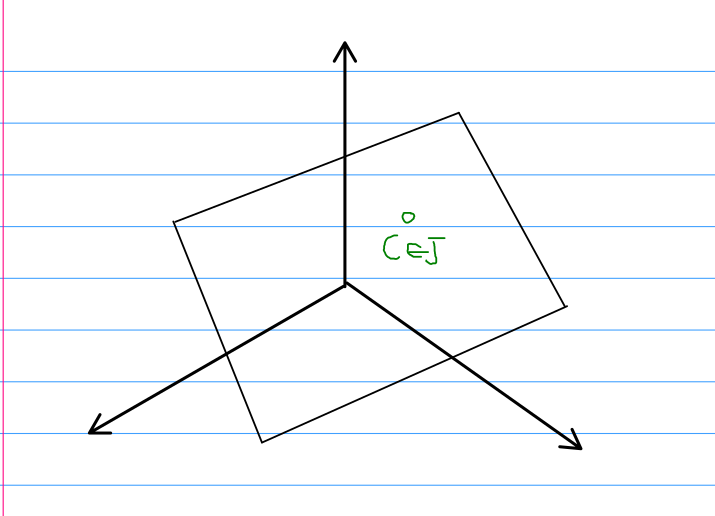
\includegraphics[width=0.3\linewidth]{figures/grass.png}
\caption{Visualizing some $J \in S_c$.}
\label{grass}
\end{figure}
Why is $S_c$ a submanifold? Consider charts on $\mathrm{Gr}$ (or $\mathrm{Gr}^-$). For $J \in \mathrm{Gr}$, choose a complement $K$, so $H = J \oplus K = H^2 _{\mathrm{DR}}(X)$. Then $\Hom _{\R}(J,K) \xrightarrow{\phi _{J,K}} \mathrm{Gr}, \theta \mapsto  \mathrm{graph}(\theta)$, where $\phi _{J,K}$ is an atlas for $\mathrm{Gr}$. Suppose now that $c \in J$, or $J \subseteq S_c$. $\phi _{J,K}$ maps $\{\theta \in \Hom(J,K) \mid \theta(c) = 0\} $ to a neighborhood of $J$ in $S_c$, i.e. we get a \emph{submanifold} chart. Since $b^+ > 0$, $\mathrm{Gr}^- \setminus S_c$ is open and dense in $\mathrm{Gr}^-$. We can look at $\bigcup_{0\neq c \in H^2_{\Z}} S_c \subseteq \mathrm{Gr}^-$, a countable union of closed submanifolds of positive codimension, and is \emph{generic}  (no idemp sets). What this tells us is that our intution that if we look at a Grassmannian and a random subspace to see how it intersects the integer lattice is that it only intersects at the origin. 

Our next step is to show that $P$ is transverse to each of the submanifolds $S_c$ where $0\neq c \in H^2_{\Z}$. This implies that $P^{-1}(S_c) \subseteq \mathcal C_r(X)$ is a closed codimensional $b^+$ submanifold (where $\mathcal C_r(X)$ is an $\infty$-dimensional manifold). This implies our theorem. Transversality means that if $P[g] \in S_c$, then $\boxed{T _{P[g]}^{\mathrm{Gr}^-}= T_{P[g]}S_c + \im D_{[g]}P}$ (the derivative of the period map). This is the technical statement that is going to be proved. Some of the proof will be next time, primarily using a Hodge theoretic calculation. First you differentiate the Hodge star with respect to the conformal structure, then you differentiate the period map. It also uses a principle from PDEs, called unique continuation for harmonic 2-forms.

